\section{Basic Extensions of the Chromosome Evolution Model}\label{sec:chromo_extensions}

In this section, we will extend the ChromEvol model in a number of ways.
First, we will examine another approach for treating chromosome number root frequencies.
This is followed by a brief example applying stochastic character mapping to chromosome evolution
models.
Then will look at jointly estimating the phylogeny and chromsome evolution,
show how to set up a BiChroM analysis, and demonstrate one way to add cladogenetic changes
to a chromosome evolution analysis.

Like before, scripts for these examples are also provided in the \RevBayes tutorial repository\footnote{\url{https://github.com/revbayes/revbayes_tutorial/tree/master/RB_Chromosome_Evolution_Tutorial/scripts}}. 
Please refer to these files to verify or troubleshoot your own scripts. 

\bigskip
\subsection{Improved Root Frequencies}\label{subsect:root_freq}

In the last example we assumed the frequency of chromosome numbers at the root of the tree
were equal. This is equivalent to assigning an extremely informative prior that all root states
are equally likely.
An alternative approach is to treat the root frequencies
as free parameters of the model and estimate them from the observed data.
In a series of unpublished simulations performed by the authors this resulted in increased accuracy of 
ancestral root chromosome numbers estimates. 


To use this approach, the \texttt{root\_frequencies} parameter must be redefined
as a stochastic node in our graphical model instead of a deterministic node.
Remove the following line from your \Rev script:
{\tt \begin{snugshade*}
\begin{lstlisting}
root_frequencies := simplex(rep(1, max_chromo + 1))
\end{lstlisting}
\end{snugshade*}}

We will instead use an uninformative flat Dirichlet prior for the root frequencies.
First, we create a vector to hold the concentration parameters for the Dirichlet
distribution. Here we set all concentration parameters to 1, which results in all
sets of probabilities being equally likely.
We then pass the vector of concentration parameters into the Dirichlet distribution
and create the stochastic node representing root frequencies.
{\tt \begin{snugshade*}
\begin{lstlisting}
root_frequencies_prior <- rep(1, max_chromo + 1)
root_frequencies ~ dnDirichlet(root_frequencies_prior)
\end{lstlisting}
\end{snugshade*}}

Next, we must specify MCMC moves for the root frequencies.
When the maximum number of chromosomes is high these parameters
can have difficulty converging.
Therefore, we use two different MCMC moves. The first is Beta Simplex move, which selects one
element of the \texttt{root\_frequencies} vector and proposes
a new value for it drawn from a Beta distribution.
The second is Element Swap Simplex move, which selects two elements
of the \texttt{root\_frequencies} vector and simply swaps their values.
{\tt \begin{snugshade*}
\begin{lstlisting}
moves[mvi++] = mvBetaSimplex(root_frequencies, alpha=0.5, weight=10)
moves[mvi++] = mvElementSwapSimplex(root_frequencies, weight=10)
\end{lstlisting}
\end{snugshade*}}
You can experiment with different weights for each MCMC move.


\medskip
\subsection{Stochastic Character Mapping of Chromosome Evolution}\label{subsect:stoch_mapping}


In \RevBayes both ancestral states and stochastic character maps can be sampled from
continuous-time Markov chain (CTMC) and state-dependent speciation and
extinction (SSE) models of character evolution.
Stochastic character maps show the timing and number of transitions
along the branches of the phylogeny, so they can be particularly useful
for chromosome evolution estimates where the timing of, for example, whole genome duplication events
might be of interest. This example is performed on a non-ultrametric tree, but
the same analysis could be performed on time-calibrated trees.

\begin{figure}[h!]
\fbox{
\begin{minipage}{\textwidth}\centering
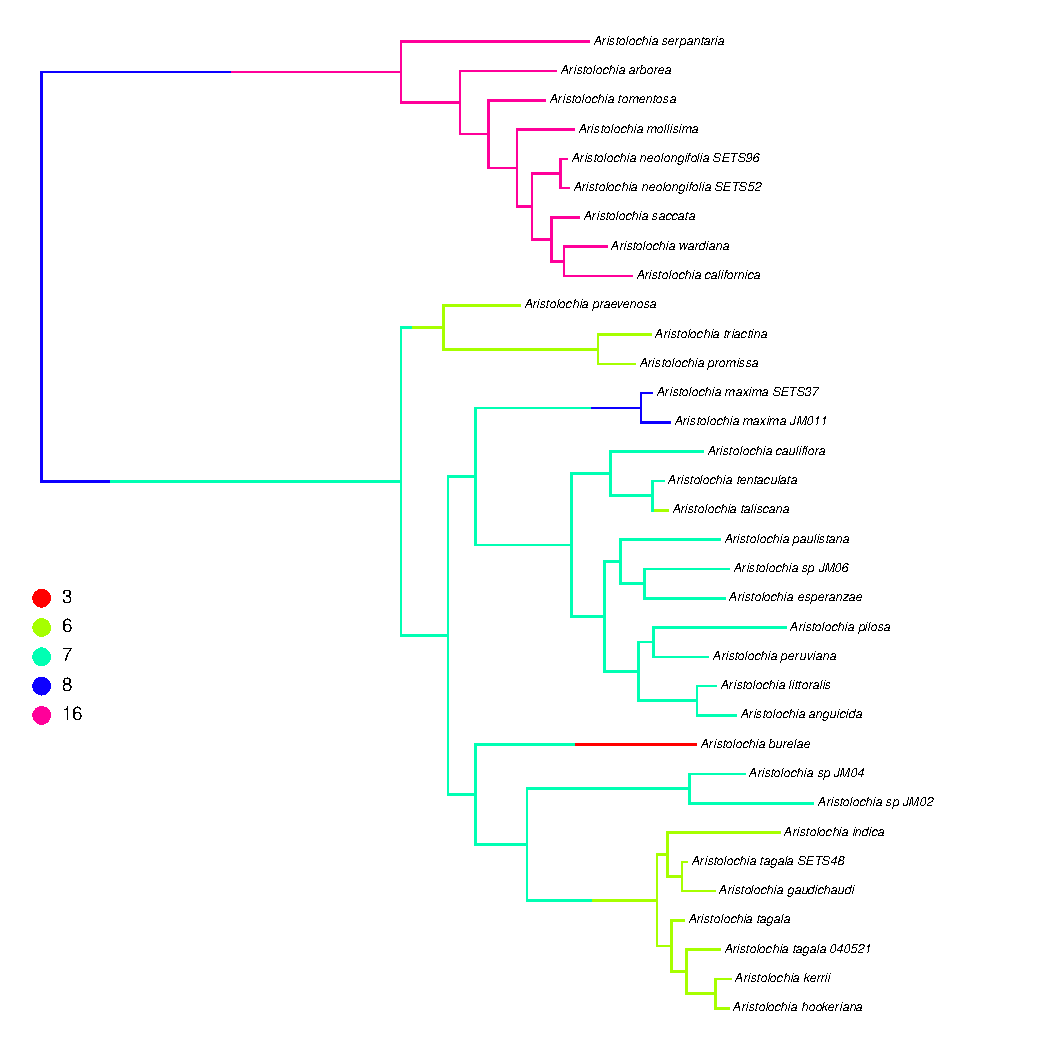
\includegraphics[width=0.92\textwidth,angle=0]{\ResourcePath figures/simmap}
    \caption{\small 
    An example of stochastic character mapping applied to chromosome number evolution using \RevBayes. Shown is the marginal maximum a posteriori chromosome evolution history of \textit{Aristolochia}
    using the simple ChromEvol analysis from Section \ref{sec:chromo_basic_analysis}.}
\end{minipage}}
\label{fig:simmap}
\end{figure}


We have already shown how to sample ancestral states above, and here we show
the few extra lines of \Rev code needed to sample stochastic character maps.
Stochastic character maps are drawn during the MCMC, so we need to include the
\texttt{mnStochasticCharacterMap} monitor.
{\tt \begin{snugshade*}
\begin{lstlisting}
monitors[4] = mnStochasticCharacterMap(ctmc=chromo_ctmc, filename="output/ChromEvol_maps.log", printgen=10)
\end{lstlisting}
\end{snugshade*}}
This monitor will create the \texttt{output/ChromEvol\_maps.log} file.
Just like the other log files, each row in this file represents a different sample from the MCMC.
Each column in the file, though, is the character history for a different node in the phylogeny.
The last column of the file is the full stochastic character map of the entire tree
in \textbf{SIMMAP} \citep{bollback2006simmap} format.
These can be plotted using the \textbf{phytools} R package \citep{revell2012phytools}.

After the MCMC, we can calculate the maximum a posteriori marginal, joint, or conditional
character history. This process is similar to the ancestral state summaries.
First we read in the stochastic character map trace.
{\tt \begin{snugshade*}
\begin{lstlisting}
anc_state_trace = readAncestralStateTrace("output/ChromEvol_simple_maps.log")
\end{lstlisting}
\end{snugshade*}}
Then we use the \texttt{characterMapTree} function. This generates two SIMMAP formatted files:
1) the maximum a posteriori character history, and 2) the posterior probabilities of the
entire character history.
{\tt \begin{snugshade*}
\begin{lstlisting}
characterMapTree(phylogeny, anc_state_trace, character_file="output/character.tree", posterior_file="output/posterior.tree", burnin=5, reconstruction="marginal")
\end{lstlisting}
\end{snugshade*}}
Figure \ref{fig:simmap} is an example stochastic character map of our \textit{Aristolochia} analysis plotted using \textbf{phytools}. 

\medskip
\subsection{Joint Estimation of Phylogeny and Chromosome Evolution}\label{subsect:joint_estimation}


In \RevBayes the chromosome evolution models can be used jointly with a model of molecular evolution 
enabling joint inference of the phylogeny and chromosome number evolution.
This enables the chromosome number analysis to take into account phylogenetic uncertainty 
and allows the chromosome numbers to help inform the phylogeny. 

Setting up a model that jointly infers chromosome evolution and phylogeny requires mostly combining
elements covered in the \textbf{Molecular Models of Character Evolution} tutorial with the
what has already been covered in Section \ref{sec:chromo_basic_analysis} of this tutorial. We will not repeat how to set up the chromosome model
component, but we'll step through what must be added to the example in Section \ref{sec:chromo_basic_analysis} above.
Furthermore, we have provided a full working example script \texttt{scripts/ChromEvol\_joint.Rev}.

\subsubsection{Reading in Molecular Data and Setting Clade Constraints}

The first major difference from the basic ChromEvol example shown above is that we must additionally
read in molecular sequence data:
{\tt \begin{snugshade*}
\begin{lstlisting}
dna_seq = readDiscreteCharacterData("data/aristolochia_matK.fasta")
\end{lstlisting}
\end{snugshade*}}
We will need some useful information about this data as well:
{\tt \begin{snugshade*}
\begin{lstlisting}
n_species = dna_seq.ntaxa()
n_sites = dna_seq.nchar()
taxa = dna_seq.names()
n_branches = 2 * n_species - 2
\end{lstlisting}
\end{snugshade*}}
Since we want to jointly infer ancestral states, we need to set an a priori
rooting constraint on our phylogeny. So here we set an ingroup and outgroup.
{\tt \begin{snugshade*}
\begin{lstlisting}
outgroup = ["Aristolochia_serpantaria", "Aristolochia_arborea", 
            "Aristolochia_wardiana", "Aristolochia_californica", 
            "Aristolochia_saccata", "Aristolochia_mollisima",
            "Aristolochia_tomentosa", "Aristolochia_neolongifolia_SETS52", 
            "Aristolochia_neolongifolia_SETS96"]
\end{lstlisting}
\end{snugshade*}}
Here we loop through each taxon and if it is not present in the outgroup
defined above we add it to the ingroup.
{\tt \begin{snugshade*}
\begin{lstlisting}
i = 1
for (j in 1:taxa.size()) {
    found = false
    for (k in 1:outgroup.size()) {
        if (outgroup[k] == taxa[j].getSpeciesName()) {
            found = true
            break
        }
    }
    if (found == false) {
        ingroup[i] = taxa[j].getSpeciesName()
        i += 1
    }
}
\end{lstlisting}
\end{snugshade*}}
And now we make the vector of clade objects to constrain our tree topology.
{\tt \begin{snugshade*}
\begin{lstlisting}
clade_ingroup = clade(ingroup)
clade_outgroup = clade(outgroup)
clade_constraints = [clade_ingroup, clade_outgroup]
\end{lstlisting}
\end{snugshade*}}

\subsubsection{Tree Model}

We will specify a uniform prior on the tree topology, and add
a MCMC move on the topology.
{\tt \begin{snugshade*}
\begin{lstlisting}
topology ~ dnUniformTopology(taxa=taxa, constraints=clade_constraints, rooted=TRUE)
moves[mvi++] = mvNNI(topology, weight=10.0)
\end{lstlisting}
\end{snugshade*}}
Next, we create a stochastic node for each branch length.
Each branch length prior will have an exponential distribution with rate 1.0.
We'll also add a simple scaling move for each branch length.
{\tt \begin{snugshade*}
\begin{lstlisting}
for (i in 1:n_branches) {
    br_lens[i] ~ dnExponential(10.0)
    moves[mvi++] = mvScale(br_lens[i], lambda=2, weight=1)
}
\end{lstlisting}
\end{snugshade*}}
Finally, build the tree by combining the topology with the branch lengths.
{\tt \begin{snugshade*}
\begin{lstlisting}
phylogeny := treeAssembly(topology, br_lens)
\end{lstlisting}
\end{snugshade*}}

\subsubsection{Molecular Substitution Model}

We'll specify the GTR substitution model applied uniformly to all sites.
Use a flat Dirichlet prior for the exchange rates.
{\tt \begin{snugshade*}
\begin{lstlisting}
er_prior <- v(1,1,1,1,1,1)
er ~ dnDirichlet(er_prior)
moves[mvi++] = mvSimplexElementScale(er, alpha=10, weight=3)
\end{lstlisting}
\end{snugshade*}}
And also a flat Dirichlet prior for the stationary base frequencies.
{\tt \begin{snugshade*}
\begin{lstlisting}
pi_prior <- v(1,1,1,1)
pi ~ dnDirichlet(pi_prior)
moves[mvi++] = mvSimplexElementScale(pi, alpha=10, weight=2)
\end{lstlisting}
\end{snugshade*}}
Now create a deterministic variable for the nucleotide substitution rate matrix.
{\tt \begin{snugshade*}
\begin{lstlisting}
Q_mol := fnGTR(er, pi)
\end{lstlisting}
\end{snugshade*}}
Create a stochastic node for the sequence evolution continuous-time Markov chain (CTMC)
and clamp the sequence data.
Note we should have two CTMC objects in this model: one for the model of molecular evolution
and one for the model of chromosome evolution.
{\tt \begin{snugshade*}
\begin{lstlisting}
dna_ctmc ~ dnPhyloCTMC(tree=phylogeny, Q=Q_mol, branchRates=1.0, type="DNA")
dna_ctmc.clamp(dna_seq)
\end{lstlisting}
\end{snugshade*}}

\subsubsection{MCMC and Summarizing Results}

We set up the MCMC just as before, except here we
need to add a file monitor to store the sampled trees.
{\tt \begin{snugshade*}
\begin{lstlisting}
monitors[2] = mnFile(filename="output/ChromEvol_joint.trees", printgen=10, phylogeny)
\end{lstlisting}
\end{snugshade*}}
Summarizing the results of the MCMC analysis are a little different.
First we will calculate the maximum a posteriori (MAP) tree.
{\tt \begin{snugshade*}
\begin{lstlisting}
treetrace = readAncestralStateTreeTrace("output/ChromEvol_joint.trees", treetype="non-clock")
map_tree = mapTree(treetrace, "output/ChromEvol_joint_map.tree")
\end{lstlisting}
\end{snugshade*}}
Now we'll summarize the ancestral chromosome numbers over the MAP tree.
Read in the ancestral state trace:
{\tt \begin{snugshade*}
\begin{lstlisting}
anc_state_trace = readAncestralStateTrace("output/ChromEvol_joint_states.log")
\end{lstlisting}
\end{snugshade*}}
Finally, calculate the marginal ancestral states from the traces over the MAP tree.
Note that this time we have to pass both the tree trace and the ancestral state
trace to the \texttt{ancestralStateTree} function.
Since we sampled a joint distribution of ancestral state histories and trees,
we sampled some ancestral states for nodes that do not exist in the MAP tree.
Therefore the ancestral state probabilities being calculated for the MAP tree
are conditional to the probability of the node existing.
{\tt \begin{snugshade*}
\begin{lstlisting}
ancestralStateTree(map_tree, anc_state_trace, treetrace, "output/ChromEvol_joint_final.tree" burnin=0.25, reconstruction="marginal")
\end{lstlisting}
\end{snugshade*}}
Like before, we can plot the results using the \RevGadgets R package.

\bigskip

\subsection{Associating Chromosome Evolution with Phenotype: BiChroM}\label{subsect:bichrom}

We may be interested in testing whether the rates of chromosome number evolution
are associated with a certain phenotype.
Here we set up a binary phenotypic character and estimate separate rates of chromosome
evolution for each state of the phenotype. 
We'll use a model that describes the joint evolution of both the
phenotypic character and chromosome evolution. This model (BiChroM) was introduced in \citet{zenil2017testing}. In RevBayes the BiChroM model can easily be extended to multistate phenotypes and/or 
hidden states, plus cladogenetic changes could be incorporated into the model.

In this example we will again use chromosome count data from \citet{ohi2006molecular} for the plant 
genus \textit{Aristolochia}. 
For the phenotype we will examine gynostemium morphology. \textit{Aristolochia} flowers have an extensively 
modified perianth that traps and eventually releases pollinators to ensure cross pollination 
(this is why the flowers resemble pipes and are commonly called Dutchman's pipes). The gynostemium 
is a reproductive organ found only in Aristolchiaceae and Orchids that consists of fused stamens 
and pistil that pollinators must interact with during pollination. The subgenus Isotrema has highly
reduced three-lobed gynostemium. Other members of \textit{Aristolochia} have gynostemium subdivided into
5 to 24 lobes. We'll test for an association of this phenotype with changes in the rates of 
chromosome evolution. 
\begin{itemize}
\item phenotype state 0 = 3 lobed gynostemium
\item phenotype state 1 = 5 t0 24 lobed gynostemium
\end{itemize}
Much of this exercise is a repeat of what was already covered in Section \ref{sec:chromo_basic_analysis},
so we will only touch on the model components that are different.
We have provided a full working example script \texttt{scripts/BiChroM.Rev}
In this example the phylogeny is assumed known. One could combine this with the exercise above
to jointly infer the phylogeny.

\begin{figure}[h!]
\fbox{
\begin{minipage}{\textwidth}\centering
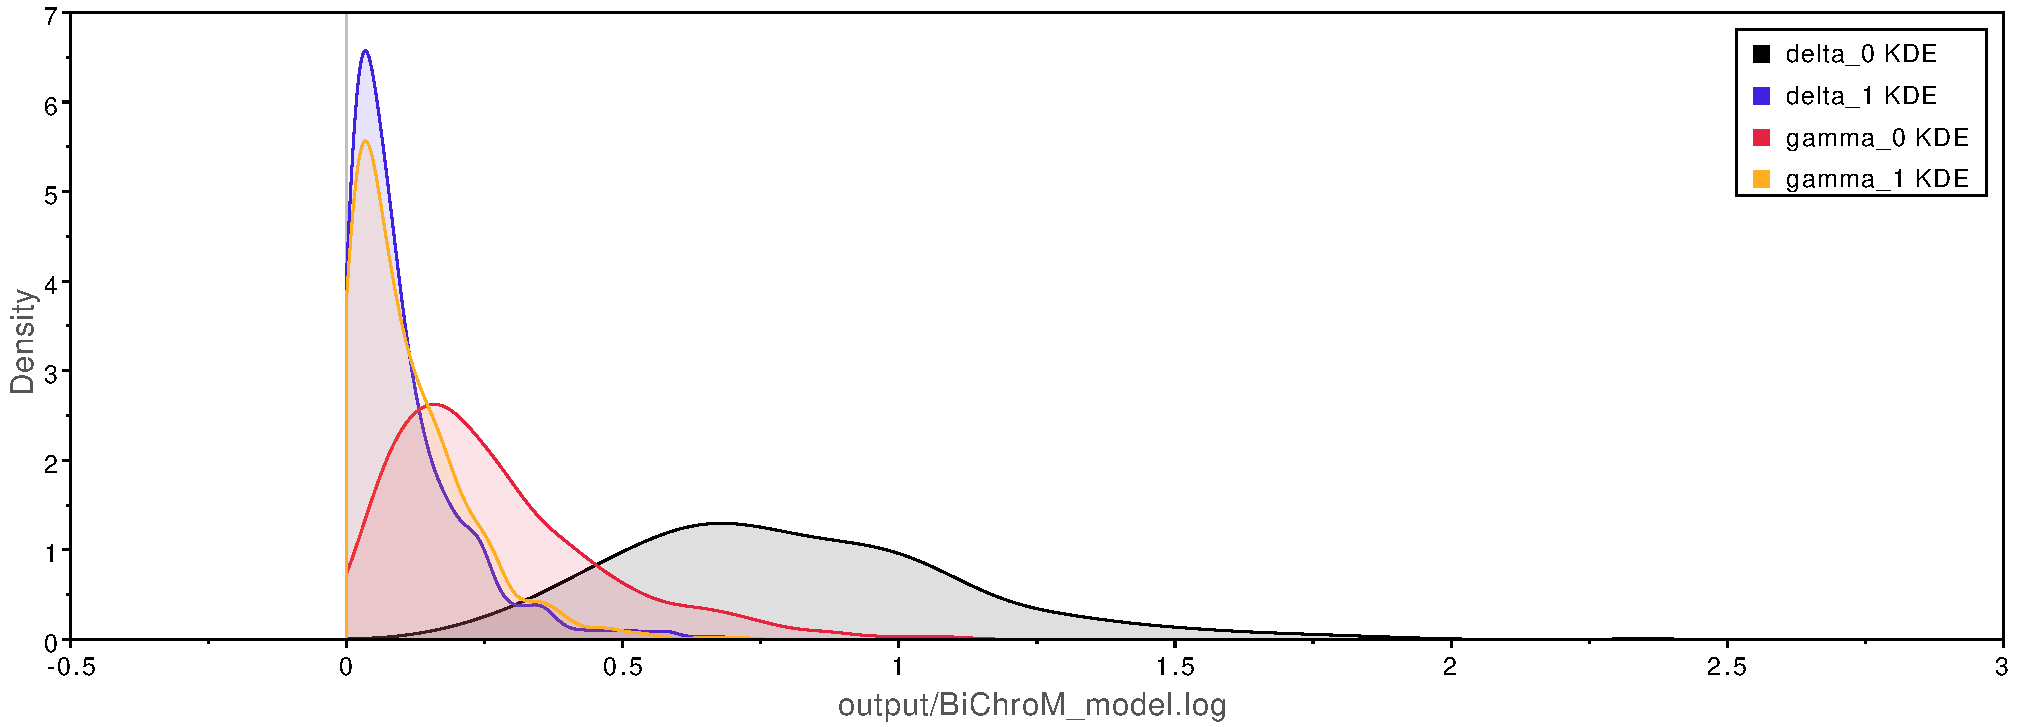
\includegraphics[width=0.92\textwidth,angle=0]{\ResourcePath figures/BiChroM_rates}
    \caption{\small Results of the example BiChroM analysis performed in \RevBayes. The rates of chromosome gains (\texttt{gamma}) and losses (\texttt{delta}) are higher for \textit{Aristolochia}
    lineages with complex gynostemium subdivided into 5 to 24 lobes (state 0) compared
    to lineages with simple 3 lobed gynostemium (state 1).}
\end{minipage}}
\label{fig:bichrom_rates}
\end{figure}

\begin{figure}[h!]
\fbox{
\begin{minipage}{\textwidth}\centering
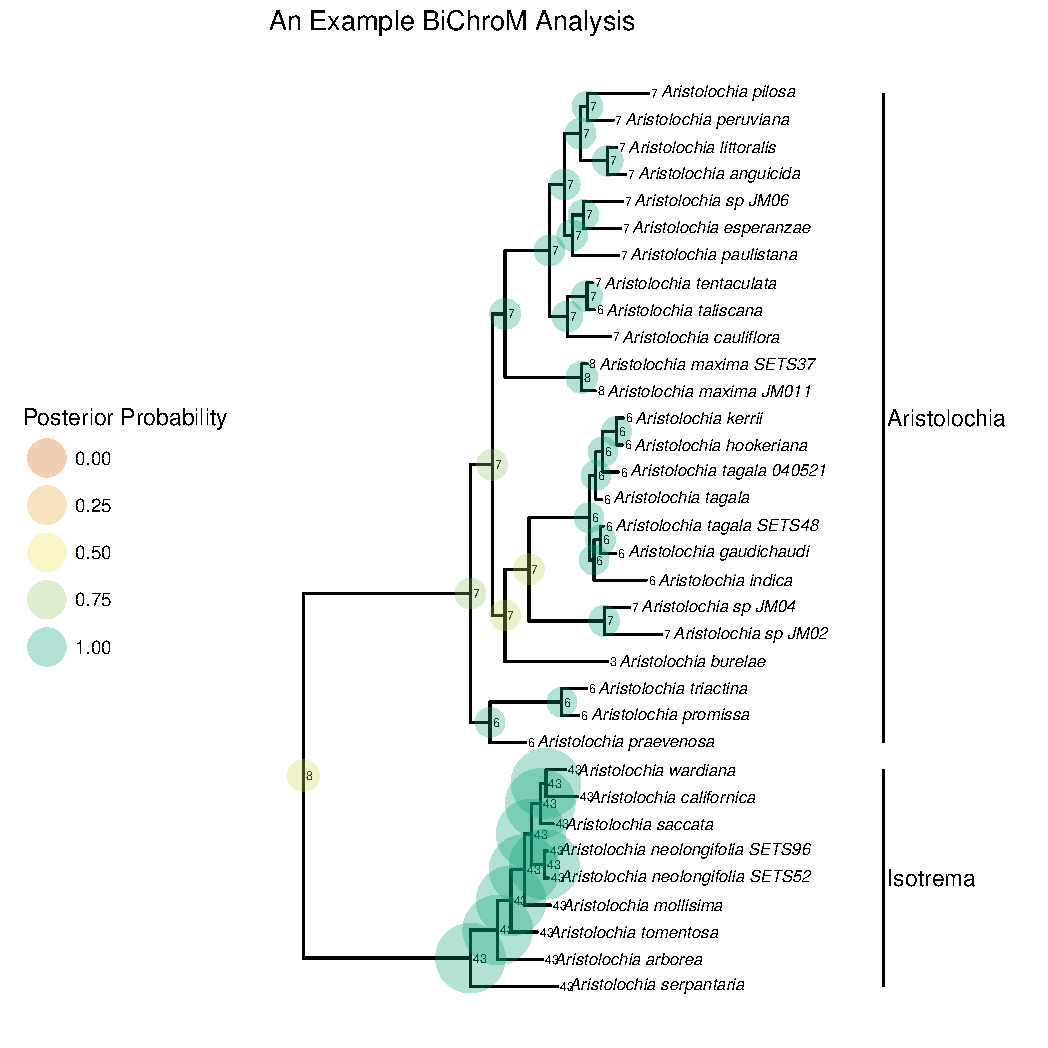
\includegraphics[width=0.92\textwidth,angle=0]{\ResourcePath figures/BiChroM}
\caption{\small Maximum a posteriori estimates of ancestral chromosome number and gynostemium morphology for \textit{Aristolochia} inferred using the BiChroM model as implemented in \RevBayes. States 1-26 represent the haploid number $n$ of chromosome for lineages
    with gynostemium subdivided in 5 to 24 lobes. States 27-52 represent the haploid number $n + 27$ of chromosomes 
    for lineages with simple 3 lobed gynostemium. The ancestral state for the common ancestor of all \textit{Aristolochia} had a haploid number $n = 8$ and more complex 5 to 24 lobed gynostemium. An evolutionary reduction to 3 lobes is inferred in the lineage leading to the extant Isotrema clade.}
\end{minipage}}
\label{fig:bichrom}
\end{figure}

\subsubsection{Setting up the BiChroM model}

The first step will be to read in the observed data. This is done as before,
with the exception that the data is set up a bit differently. The data matrix
must now represent both the observed chromosome counts \textit{and} the observed
phenotype. So in this file states 1-26 represent the haploid number $n$ of chromosome for lineages 
with gynostemium subdivided in 5 to 24 lobes, and states 27-52 represent the haploid number $n + 27$
for lineages with simple 3 lobed gynostemium.
Note the \texttt{stateLabels} argument must now be set to 2 times the maximum number of chromosomes.
{\tt \begin{snugshade*}
\begin{lstlisting}
chromo_data = readCharacterDataDelimited("data/aristolochia_bichrom_counts.tsv", stateLabels=2*(max_chromo + 1), type="NaturalNumbers", delimiter="\t", headers=FALSE)
\end{lstlisting}
\end{snugshade*}}
Like before, we'll use exponential priors to model the rates of polyploidy and 
dysploidy events along the branches of the phylogeny
However, here we set up two rate parameters for each type of chromosome change --
one for phenotype state 0 and one for phenotype state 1.
{\tt \begin{snugshade*}
\begin{lstlisting}
gamma_0 ~ dnExponential(10.0)
gamma_1 ~ dnExponential(10.0)
delta_0 ~ dnExponential(10.0)
delta_1 ~ dnExponential(10.0)
rho_0 ~ dnExponential(10.0)
rho_1 ~ dnExponential(10.0)
\end{lstlisting}
\end{snugshade*}}
Add MCMC moves for each of the rates.
{\tt \begin{snugshade*}
\begin{lstlisting}
mvi = 1
moves[mvi++] = mvScale(gamma_0, lambda=1, weight=1)
moves[mvi++] = mvScale(delta_0, lambda=1, weight=1)
moves[mvi++] = mvScale(rho_0, lambda=1, weight=1)
moves[mvi++] = mvScale(gamma_1, lambda=1, weight=1)
moves[mvi++] = mvScale(delta_1, lambda=1, weight=1)
moves[mvi++] = mvScale(rho_1, lambda=1, weight=1)
\end{lstlisting}
\end{snugshade*}}
Now we create the rate matrix for the chromosome evolution model.
We will set up two rate matrices, one for each phenotype state.
{\tt \begin{snugshade*}
\begin{lstlisting}
Q_0 := fnChromosomes(max_chromo, gamma_0, delta_0, rho_0)
Q_1 := fnChromosomes(max_chromo, gamma_1, delta_1, rho_1)
\end{lstlisting}
\end{snugshade*}}
Again, we could have include the rate of demi-polyploidization \texttt{eta}
and rate modifiers like this:
{\tt \begin{snugshade*}
\begin{lstlisting}
Q_0 := fnChromosomes(max_chromo, gamma_0, delta_0, rho_0, eta_0, gamma_l_0, delta_l_0) 
Q_1 := fnChromosomes(max_chromo, gamma_1, delta_1, rho_1, eta_1, gamma_l_1, delta_l_1) 
\end{lstlisting}
\end{snugshade*}}
Now we create the rates of transitioning between phenotype states.
Any model could be used (all rates equal models, Dollo models, etc.)
but here we estimate a different rate for each transition between states 0 and 1.
{\tt \begin{snugshade*}
\begin{lstlisting}
q_01 ~ dnExponential(10.0)
q_10 ~ dnExponential(10.0)
moves[mvi++] = mvScale(q_01, lambda=1, weight=1)
moves[mvi++] = mvScale(q_10, lambda=1, weight=1)
\end{lstlisting}
\end{snugshade*}}
And finally we create the transition rate matrix \texttt{Q\_b} 
for the joint model of phenotypic and chromosome evolution.
First we will initialize the matrix with all zeros:
{\tt \begin{snugshade*}
\begin{lstlisting}
s = Q_0[1].size()
for (i in 1:(2 * s)) {
    for (j in 1:(2 * s)) {
        Q[i][j] := 0.0
    }
}
\end{lstlisting}
\end{snugshade*}}
And now we populate the matrix with the transition rates.
{\tt \begin{snugshade*}
\begin{lstlisting}
for (i in 1:(2 * s)) {
    for (j in 1:(2 * s)) {
        if (i <= s) {
            if (j <= s) {
                if (i != j) {
                    # chromosome changes within phenotype state 0
                    Q[i][j] := abs(Q_0[i][j])
                }
            } else {
                if (i == (j - s)) {
                    # transition from phenotype state 0 to 1
                    Q[i][j] := q_01
                }
            }
        } else {
            if (j <= s) {
                if (i == (j + s)) {
                    # transition from phenotype state 1 to 0
                    Q[i][j] := q_10
                }
            } else {
                if (i != j) {
                    # chromosome changes within phenotype state 1
                    k = i - s
                    l = j - s
                    Q[i][j] := abs(Q_1[k][l])
                }
            }
        }
    }
}
Q_b := fnFreeK(Q, rescaled=false)
\end{lstlisting}
\end{snugshade*}}
The rest of the analysis is essentially
the same as in Section \ref{sec:chromo_basic_analysis}. Just make sure
to pass the \texttt{Q\_b} matrix into the CTMC object.

\subsubsection{BiChroM Analysis Results}

In Figure \ref{fig:bichrom_rates} the rates of
chromosome gains and losses for each of the phenotype states are plotted.
\textit{Aristolochia} lineages with complex gynostemium subdivided into many lobes
have higher rates of dysploid changes than lineages with simple 3-lobed gynostemium.
In Figure \ref{fig:bichrom} the marginal maximum a posteriori estimates of ancestral
chromosome number and gynostemium morphology are plotted.
From this we can see that an evolutionary reduction occured on the lineage
leading to the Isotreme clade. The common ancestor for all
\textit{Aristolochia} is inferred to have complex many lobed
gynostemium which was reduced to a more simple 3-lobed form in Isotrema.  




\subsection{Incorporating Cladogenetic and Anagenetic Chromosome Changes}\label{subsect:clado_simple}

Changes in chromosome number can increase reproductive isolation and may drive the diversification
of some lineages \citep{stebbins1971chromosomal}. 
To test for the association
of chromosome changes with speciation we must extend our models to incorporate cladogenetic
changes. Cladogenetic changes are changes that occur only at lineage splitting events.
All the models of chromosome evolution we have examined so far model
only anagenetic changes, changes that occur within a lineage. 

We introduce here a simple model of cladogenetic change that handles cladogenetic events
similarly to the widely used Dispersal-Extinction-Cladogenesis \citep[DEC;][]{ree08} 
models of biogeographic range evolution.
A major limitation of such models is that they only model cladogenetic changes
at the observed speciation events on the phylogeny.
Many other unobserved speciation events likely occurred, but are not present
in the reconstructed phylogeny due to incomplete taxon sampling and lineages
going extinct. This can bias the relative rates of anagenetic and cladogenetic change.
In Section \ref{sec:chromosse_intro} we will introduce the
ChromoSSE model, which reduces this bias by explicitly modeling unobserved speciation events but at the
cost of additional model complexity.

Much of this exercise is a repeat of what was already covered in Section \ref{sec:chromo_basic_analysis},
so we will only touch on the model components that must be changed to incorporate cladogenetic
changes.
We have provided a full working example script \texttt{scripts/ChromEvol\_clado.Rev}

\subsubsection{A Simple Cladogenetic Model}

\begin{figure}[h!]
\fbox{
\begin{minipage}{\textwidth}\centering
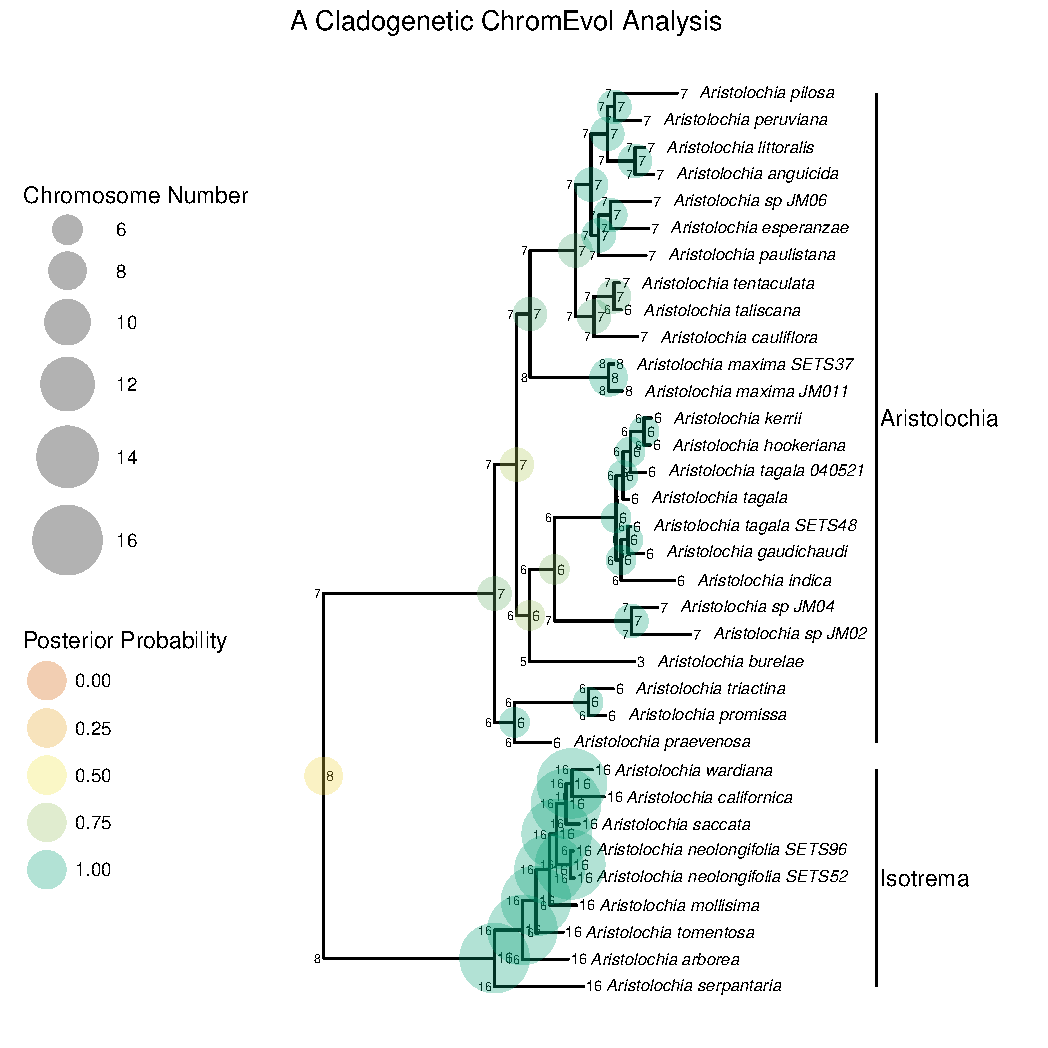
\includegraphics[width=0.92\textwidth,angle=0]{\ResourcePath figures/ChromEvol_clado}
\caption{\small Maximum a posteriori ancestral chromosome numbers for \textit{Aristolochia}
    estimated using a simple cladogenetic and anagenetic chromosome evolution model.
    The start states of each lineage (the state after cladogenesis) are plotted
    on the 'shoulders' of each lineage, and show where cladogenetic events occurred.
    This example analysis did not fully converge and shows a very high number of cladogenetic events.}
\end{minipage}}
\label{fig:chromevol_clado}
\end{figure}

The anagenetic transition rate matrix should be set up just as before.
The cladogenetic changes, though, are modeled as a vector of probabilities 
that sum up to 1 (a simplex). Each element of the vector is the 
probability of a certain type of cladogenetic event occurring.
To set this up, we'll first draw a 'weight' for each type of 
cladogenetic event from an exponential distribution. To keep the
example simply we are excluding cladogenetic demi-polyploidization.
We then pass each 'weight' into a simplex to create the vector
of probabilities.
{\tt \begin{snugshade*}
\begin{lstlisting}
clado_no_change_pr ~ dnExponential(10.0)
clado_fission_pr ~ dnExponential(10.0)
clado_fusion_pr ~ dnExponential(10.0)
clado_polyploid_pr ~ dnExponential(10.0)
clado_demipoly_pr <- 0.0
clado_type := simplex([clado_no_change_pr, clado_fission_pr, clado_fusion_pr, clado_polyploid_pr, clado_demipoly_pr])
\end{lstlisting}
\end{snugshade*}}
The function \texttt{fnChromosomesCladoProbs} 
produces a matrix of cladogenetic probabilities. This is a very
large and sparse 3 dimensional matrix that contains the transition probabilities 
of every possible state of the parent lineage transitioning to every possible 
combination of states of the two daughter lineages.
{\tt \begin{snugshade*}
\begin{lstlisting}
clado_prob := fnChromosomesCladoProbs(clado_type, max_chromo)
\end{lstlisting}
\end{snugshade*}}
We can't forget to add moves for each cladogenetic event:
{\tt \begin{snugshade*}
\begin{lstlisting}
moves[mvi++] = mvScale(clado_no_change_pr, lambda=1.0, weight=2)
moves[mvi++] = mvScale(clado_fission_pr, lambda=1.0, weight=2)
moves[mvi++] = mvScale(clado_fusion_pr, lambda=1.0, weight=2)
moves[mvi++] = mvScale(clado_polyploid_pr, lambda=1.0, weight=2)
\end{lstlisting}
\end{snugshade*}}
Now we can create the cladogenetic CTMC model.
We must pass in both the \texttt{Q} matrix that represents the anagenetic changes,
and the \texttt{clado\_probs} matrix that represents the cladogenetic changes.
{\tt \begin{snugshade*}
\begin{lstlisting}
chromo_ctmc ~ dnPhyloCTMCClado(Q=Q, tree=phylogeny, cladoProbs=clado_prob, rootFrequencies=root_frequencies, type="NaturalNumbers", nSites=1)
\end{lstlisting}
\end{snugshade*}}
Most of the rest of the analysis is the same.
For the ancestral state monitor we want to be sure to specify 
\texttt{withStartState=true} so that we sample the states both at
start and end of each branch. This enables us to reconstruct cladogenetic events.
{\tt \begin{snugshade*}
\begin{lstlisting}
monitors[2] = mnJointConditionalAncestralState(filename="output/ChromEvol_clado_anc_states.log", printgen=10, tree=phylogeny, ctmc=chromo_ctmc, withStartStates=true, type="NaturalNumbers")
\end{lstlisting}
\end{snugshade*}}
When summarizing the ancestral state results we also want to specify 
\texttt{include\_start\_states=true} so that we summarize the cladogenetic changes.
{\tt \begin{snugshade*}
\begin{lstlisting}
ancestralStateTree(phylogeny, anc_state_trace, "output/ChromEvol_clado_final.tree", include_start_states=true, burnin=0.25, reconstruction="marginal")
\end{lstlisting}
\end{snugshade*}}
And that's it!
Figure \ref{fig:chromevol_clado} shows the ancestral state estimates plotted on the
tree. The start states of each lineage (the state after cladogenesis) are plotted
on the 'shoulders' of each lineage.
You may want to try stochastic character mapping for a different and possibly better
visualization of cladogenetic and anagenetic changes.


\newpage
